% This file contains examples for different tex-snippets. Since they're only examples, this would must not be included in any final document.

\chapter{Demo-chapter}

Lorem ipsum dolor sit amet, consectetur adipiscing elit. Ut efficitur maximus diam, aliquam ultricies tortor semper non. Sed lobortis dolor vel facilisis auctor. In metus ante, venenatis at accumsan non, ultricies in ante. Maecenas placerat felis ipsum, nec luctus ligula pellentesque eu. Nulla dapibus neque cursus augue varius, in ultricies dolor malesuada. In bibendum imperdiet nisi, ut feugiat neque pellentesque eget. Nulla tortor mauris, sodales id arcu quis, aliquet pulvinar est. Praesent lobortis faucibus magna quis vestibulum.

\section{Demo-sub-chapter}

Vestibulum rhoncus eget mi ac accumsan. Praesent metus nisi, pellentesque ut nunc sit amet, eleifend mattis tellus. Nullam rhoncus tellus nec augue laoreet, quis cursus nisl dictum. Quisque scelerisque nisl et volutpat hendrerit. Nunc cursus nibh dolor, venenatis pulvinar dui lacinia sit amet. Aliquam diam sapien, consectetur sodales tempor non, eleifend a sem. Pellentesque quam tortor, placerat a enim vitae, porta laoreet neque.

\section{Second-demo-sub-chapter}

\marginpar{Sidenotes for the second demo-sub-chapter}

Suspendisse lectus lacus, eleifend et velit ut, luctus elementum nisl. Nunc rhoncus ultricies metus, in feugiat odio tempor nec. Nulla rutrum, urna eu suscipit ornare, nisl metus venenatis neque, ut consectetur nulla urna vitae mauris. Aliquam ac neque ut velit ultrices mattis. Vestibulum sodales vulputate arcu quis congue. Maecenas nec odio tempus, fringilla nisl laoreet, condimentum felis. Quisque auctor quam vel augue blandit vehicula.

% highlighting and text formatting
\hl{Higlighting}, \st{striking-through}, \ul{underlining} and several more simple formatting opportunities are possible.

% emphasizing
\emph{Emphasizing} text is also possible.

% long hyphen
A long hyphen --- can be written as well.

% links
Insert links like this: \url{https://github.com/thetillhoff/master-thesis}

% Acronyms and glossary
Acronyms are written down as: \gls{yamlacr}. Following occurences are then displayed as: \gls{yamlacr}.
\newline
Entries of the glossary are written down as: \gls{yaml}. Following occurences are then displayed as: \gls{yaml}.

% inline code
In this line you can see an example for \mintinline[bgcolor=lightgray,breaklines]{bash}{inline code}.

% codeblock
Here follows a complete codeblock with caption and red highlighting:

\begin{listing}[H]\begin{addmargin}[2em]{2em}\begin{minted}[linenos,bgcolor=lightgray,breaklines,escapeinside=||]{yaml}
# Folgende unterschiedliche Einrückung derselben Ebene ist in YAML erlaubt:
firstlevel1:
  secondlevel1: somevalue
  secondlevel2: anothervalue
firstlevel2:
    secondlevel3: alsoanothervalue
    secondlevel4: andonemore
# Folgende unterschiedliche Einrückung derselben Ebene ist in YAML nicht erlaubt:
firstlevel3:
|\setlength{\fboxsep}{0pt}\colorbox{red}{\strut{  secondlevel5: hello}}|
    secondlevel6: world
    secondlevel7: exclamationmark
\end{minted}
\caption{\gls{yaml} Einrückungen}
\label{code:yamlindentation}
\end{addmargin}
\end{listing}

and one without caption and highlighting:
\begin{addmargin}[2em]{2em}
\mint[bgcolor=lightgray]{js}|"group":["John Smith","Jane Smith"]|
\end{addmargin}

Use \newline \textbackslash newline for newlines and \clearpage \textbackslash clearpage for pagebreaks \\
(\textbackslash cleardoublepage is used to also skip the next page as well if it is odd numbered and the document is set to twosided)

Different vertical spaces are:
\newline\smallskip
smallskip,
\newline\medskip
medskip and
\newline\bigskip
bigskip

Text can be on the left side \hfill \textbackslash hfilland on the right side.

\vfill \textbackslash vfill makes text to appear at the bottom of a page.

% unordered list
An unordered list:
\begin{itemize}
  \item First item
  \item Second item
  \item Three dots either as ... or as \ldots
\end{itemize}

% unordered list
An unordered list with specific seperation space:
\begin{itemize}
  \setlength{\itemsep}{0pt}
  \item First item
  \item Second item
\end{itemize}

% ordered list
An ordered list, where the numbers start after 3:
\begin{enumerate}
  \setcounter{enumi}{3}
  \item Some
  \item example
  \item content
\end{enumerate}


% image
Now, an image follows - also with caption:

\begin{figure}[H]
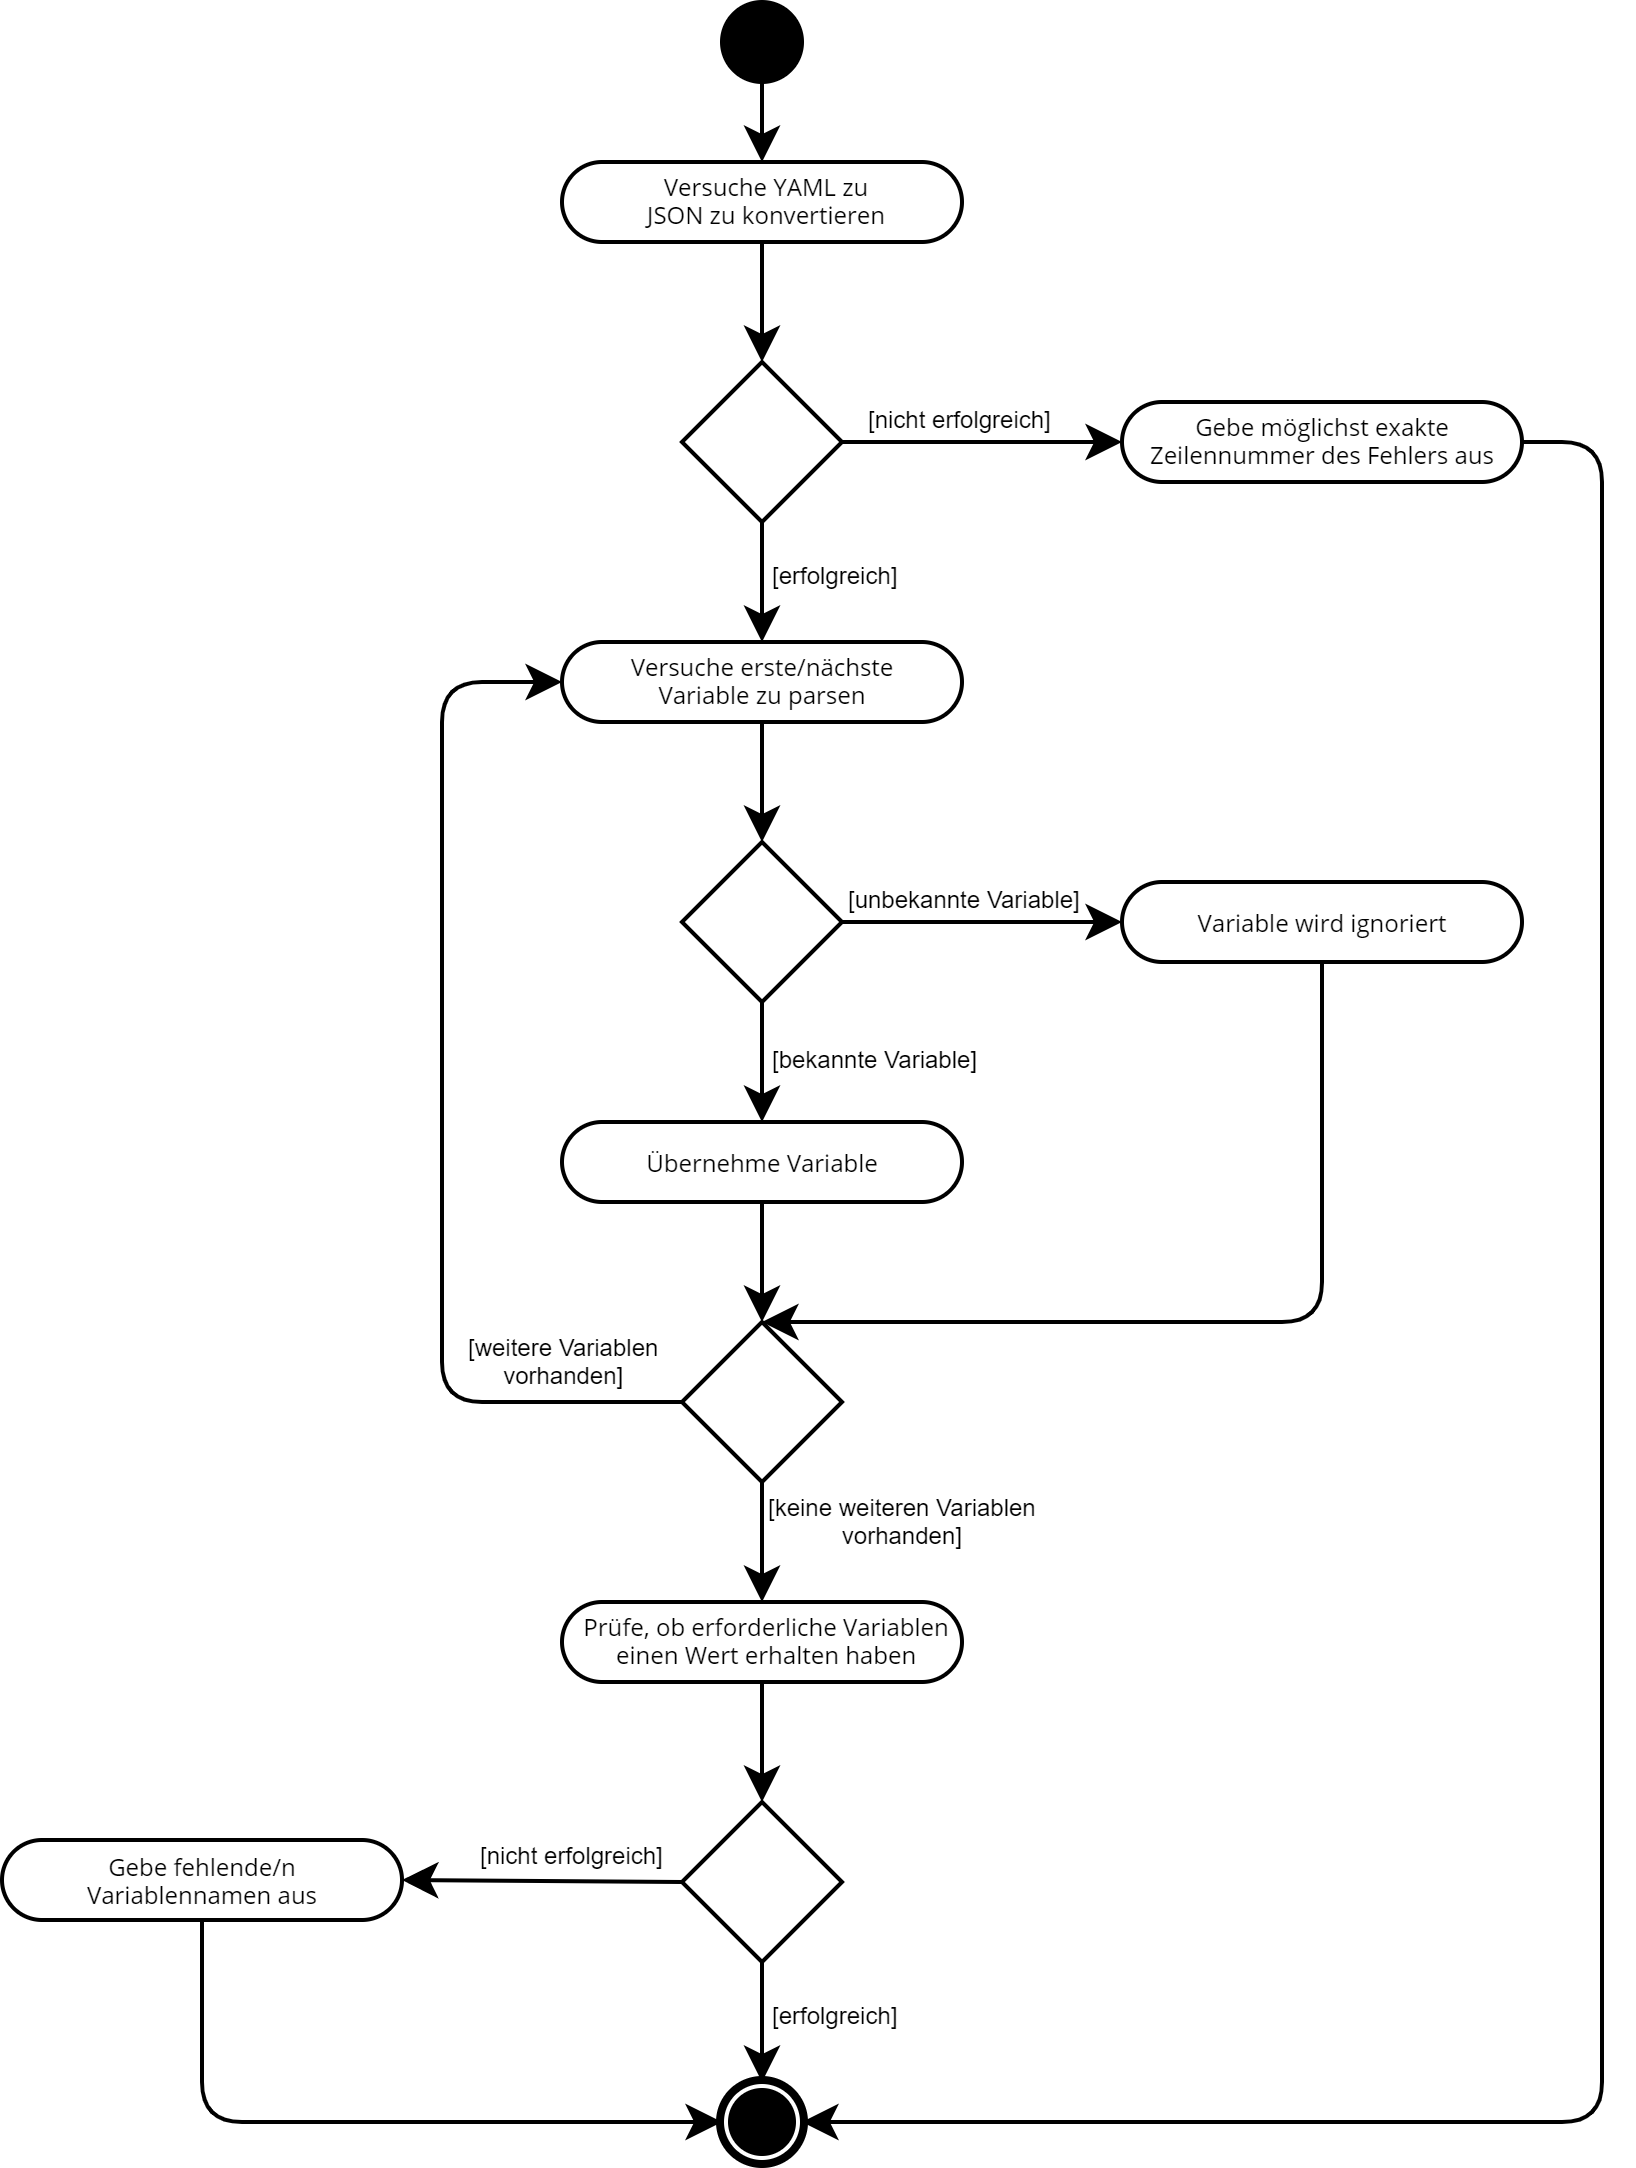
\includegraphics[width=14cm]{kubernetes_errorhandling}
\centering
\caption{UML-Aktivitätsdiagramm: Verarbeitung von an Helm und Kubernetes übergebenen Variablen}
\label{image:kubernetes_errorhandling}
\end{figure}
